\documentclass[a4paper]{ctexart}
\usepackage[top=3cm, bottom=2cm]{geometry}
\usepackage{graphicx}
\usepackage{subcaption}
\usepackage{amsmath}
\usepackage{amssymb}
\usepackage{xcolor}
\usepackage{url}
\usepackage{booktabs}
\usepackage{multirow}
%\usepackage{hyperref}
\usepackage[hidelinks]{hyperref} % 加载 hyperref 并隐藏链接边框

%\usepackage[utf8]{inputenc}
%\usepackage[ngerman]{babel} % 加载德语支持

% booktabs 提供 \toprule, \midrule, \bottomrule 等表格命令
% (booktabs 已在第9行加载，此处不再重复)

% 定义占位命令以避免未定义控制序列错误
%\newcommand{\placeholderspace}{}
\usepackage{fancyhdr} % 导入fancyhdr宏包
\usepackage{lipsum}   % 仅用于生成示例文本
\usepackage{float}    % 提供 H 浮动位置选项

% 设置页面样式为fancy
\pagestyle{fancy}
% 自定义页眉内容
\fancyhead[L]{} % 左侧页眉
\fancyhead[C]{\textbf{Physics-experiment Reporting Letter:\\Thermal Light Correlation Imaging}} % 中间页眉
\fancyhead[R]{} % 右侧页眉
% 自定义页脚内容
\fancyfoot[L]{} % 左侧页脚
\fancyfoot[C]{\thepage} % 中间页脚显示页码
\fancyfoot[R]{} % 右侧页脚
% 改变页眉线的粗细
\renewcommand{\headrulewidth}{1.4pt}
% 改变页脚线的粗细
\renewcommand{\footrulewidth}{0pt}

\title{热光鬼关联成像}
\author{实验人：学生\qquad 学号：[学号已脱敏]\qquad 指导教师：张耀峰}
\date{实验日期：2026.5.22}

\begin{document}
    
    \maketitle
    
\begin{abstract}

本实验利用旋转毛玻璃产生的类热光源，研究热光场的强度关联性质及其关联成像现象。实验首先采用 Hanbury Brown-Twiss（HBT）装置测量热光的时间关联特性，获得热光场的关联时间；随后利用分束镜将热光分为参考臂和取样臂，通过关联测量重建双孔物体的空间分布，并验证热光关联成像所满足的高斯成像公式。实验结果表明，虽然参考臂和取样臂中的单独光强分布均无法直接反映物体信息，但通过二阶强度关联测量能够恢复物体的像。实验进一步说明，关联成像并非量子纠缠光所独有，经典热光源同样可以实现鬼成像现象。\\

\textbf{关键词：热光关联成像\quad HBT实验\quad 二阶关联函数\quad 鬼成像}

\end{abstract}
    
\section{引言}

传统光学成像依赖于光场强度的直接测量，即利用探测器记录物体透射或反射后的光强分布，从而重建物体的空间结构。然而在某些情况下，单独测量光强并不能获得完整的空间信息，光场不同位置之间的关联性质反而携带了更丰富的信息。

1995年，Shih等人利用自发参量下转换产生的纠缠光子对首次实现了鬼成像（Ghost Imaging）。实验发现，即使探测器本身并不具有空间分辨能力，通过对两路光场进行符合测量，仍然能够恢复出物体的图像。这一结果最初被认为是量子纠缠所特有的现象。

随后，人们发现经典热光源同样具有二阶关联特性。理论研究表明，热光场在空间上存在统计关联，通过测量不同位置光强之间的关联函数，也能够获得物体的信息。因此，关联成像并不一定依赖量子纠缠，而可以通过经典统计关联实现。

本实验利用旋转毛玻璃产生的类热光源，首先测量热光场的时间关联特性，然后构建热光关联成像系统，对双孔物体进行关联成像实验，从而验证热光场的空间关联性质及热光关联成像理论。

\section{原理}
\subsection{热光场及其统计性质}

热光是一种典型的随机光场，其振幅与相位均随时间发生随机变化。自然界中的白炽灯、恒星辐射等均属于热光源。

本实验中采用激光照射旋转毛玻璃的方法产生类热光源。激光经过毛玻璃表面的随机微结构后，不同位置散射光之间产生随机相位差，在观察面形成随机散斑（Speckle）分布。随着毛玻璃不断转动，散斑图样随时间变化，因此获得了具有热光统计性质的随机光场。

虽然热光的平均光强保持稳定，但瞬时光强存在明显涨落。正是这种涨落导致了不同位置之间出现统计关联，从而成为热光关联成像的物理基础。

\subsection{光场关联函数}

为了描述随机光场的统计性质，引入关联函数的概念。

一阶关联函数定义为

\begin{equation}
G^{(1)}
=
\left<
E^*(r_1,t_1)
E(r_2,t_2)
\right>,
\end{equation}

它反映不同空间位置或不同时刻电场之间的关联程度。

传统干涉实验测量的正是一阶关联性质，因此一阶关联函数又称场关联函数。

对于热光关联成像，更重要的是二阶关联函数

\begin{equation}
G^{(2)}
=
\left<
I(r_1,t_1)
I(r_2,t_2)
\right>.
\end{equation}

二阶关联函数描述两个位置光强涨落之间的相关程度。

若定义归一化二阶关联函数

\begin{equation}
g^{(2)}
=
\frac
{\left<I_1I_2\right>}
{\left<I_1\right>\left<I_2\right>},
\end{equation}

则对于理想热光源有

\begin{equation}
g^{(2)}(0)=2.
\end{equation}

这一现象称为光子聚束（Photon Bunching）效应。

\subsection{HBT实验原理}

1956年，Hanbury Brown 和 Twiss 提出了著名的 HBT 实验。

实验装置利用分束镜将热光分为两路，分别由探测器
$D_1$
和
$D_2$
接收。

通过计算两探测器输出信号之间的相关函数

\begin{equation}
G^{(2)}(\tau)
=
\left<
I_1(t)
I_2(t+\tau)
\right>,
\end{equation}

可以获得热光场的时间关联特性。

当时间延迟
$\tau=0$
时，两探测器接收到的光强涨落最为相关，因此关联函数达到最大值。

随着时间延迟不断增加，光场逐渐失去关联，

\begin{equation}
g^{(2)}(\tau)
\rightarrow
1.
\end{equation}

关联函数由峰值衰减到背景值所对应的时间尺度称为关联时间。

实验中通过测量
$g^{(2)}(\tau)$
曲线即可获得热光源的关联时间，并进一步分析热光场的统计性质。

\subsection{热光关联成像原理}

热光关联成像系统由参考臂和取样臂组成。

热光经过分束镜后被分为两束光，其中参考臂中的光直接传播至扫描探测器，而取样臂中的光经过待测物体后由桶探测器收集。

由于热光本身具有随机涨落特性，因此单独观察任一路探测器的输出信号均无法直接获得物体信息。

对于参考臂，

\begin{equation}
I_R(r)
\end{equation}

只表现为随机散斑分布；

对于取样臂，

\begin{equation}
I_T
\end{equation}

则仅包含物体透射后的总光强信息。

然而两路光均来源于同一热光源，因此保留了统计关联。

通过计算

\begin{equation}
G^{(2)}(r)
=
\left<
I_R(r)I_T
\right>,
\end{equation}

可以提取出两路光场共同携带的信息。

理论分析表明，当系统满足特定几何关系时，

\begin{equation}
\frac1{z_2-z_1}
+
\frac1{z_3}
=
\frac1f,
\end{equation}

关联函数可近似写为

\begin{equation}
G^{(2)}
\propto
|T(r)|^2,
\end{equation}

其中
$T(r)$
为物体透射函数。

因此参考臂扫描探测器获得的关联分布能够重建物体图像。

值得注意的是，参考臂中的光从未通过物体，但最终仍能够恢复物体信息，因此这一现象被称为鬼成像（Ghost Imaging）。

热光关联成像实验说明，鬼成像并非量子纠缠光所独有，经典热光源同样能够实现关联成像。

\section{实验}

\subsection{实验仪器}

实验装置主要包括半导体激光器、旋转毛玻璃、分束镜、会聚透镜、双孔物体、CCD探测器、桶探测器（Bucket Detector）、相关器、数字示波器、数据采集系统以及计算机等。半导体激光器提供稳定的单色相干光源，旋转毛玻璃用于将激光转化为具有热光统计性质的随机散斑场；分束镜将热光分为参考臂与测试臂两路；CCD用于记录参考臂中的空间光强分布，而桶探测器用于收集通过物体后的总光强信号；相关器和计算机负责完成二阶关联函数的计算与图像重建。

\subsection{热光场关联时间测量}

首先开启激光器并预热，使输出功率达到稳定状态。调节光路使激光束垂直照射旋转毛玻璃，在观察屏上可以看到明显的散斑图样。启动毛玻璃电机后，散斑图样随时间不断变化，从而形成动态热光源。

利用分束镜将热光分为两路，并分别由两个光电探测器接收。探测器输出信号经放大后输入数字相关器，通过测量两个探测器输出信号之间的时间关联函数获得热光场的统计性质。

实验过程中调节相关器的时间延迟窗口，记录归一化二阶关联函数
\[
g^{(2)}(\tau)
\]
随时间延迟 $\tau$ 的变化曲线。理论上，当时间延迟趋近于零时，关联函数达到最大值；随着时间延迟增加，关联函数逐渐衰减至背景值附近。

测量完成后，对关联曲线进行拟合，得到热光场的关联时间，并分析毛玻璃转速与关联时间之间的关系。

\subsection{热光关联成像实验}

在测试臂中放置双孔物体作为待成像目标，并按照实验要求调整各光学元件位置，使系统满足关联成像条件。调节透镜焦距及光路距离，使参考臂和测试臂中的光场能够保持良好的空间关联。

测试臂中的光经过双孔物体后由桶探测器接收。桶探测器不具备空间分辨能力，仅记录透过物体后的总光强信息。与此同时，参考臂中的CCD记录每一时刻对应的随机散斑分布。

在数据采集过程中，连续记录大量散斑图像及对应的桶探测器输出信号。由于单次曝光只能得到随机散斑分布，因此无法直接观察到物体信息，需要通过统计平均的方法提取关联信号。

实验利用计算机对参考臂光强分布与桶探测器输出进行二阶关联运算：
\[
G^{(2)}(x,y)
=
\langle I_R(x,y)I_B\rangle
-
\langle I_R(x,y)\rangle
\langle I_B\rangle .
\]

随着采样次数不断增加，随机噪声逐渐被平均掉，而参考臂与测试臂之间的关联信息不断累积，最终重建出双孔物体的空间结构。

为了研究采样次数对成像质量的影响，实验分别选取不同数量的散斑图像进行重建，对比分析图像的信噪比和分辨率变化情况。实验结束后保存原始散斑数据及重建结果，用于后续分析处理。
\section{结果与分析讨论}

\subsection{热光关联长度测量}

首先利用 Hanbury Brown--Twiss（HBT）实验装置测量热光场的二阶关联函数。固定探测器 D$_2$ 的位置，沿横向移动探测器 D$_1$，记录不同位置处的二阶关联函数 $g^{(2)}(x)$，测量结果如图所示。

\begin{figure}[htbp]
    \centering
    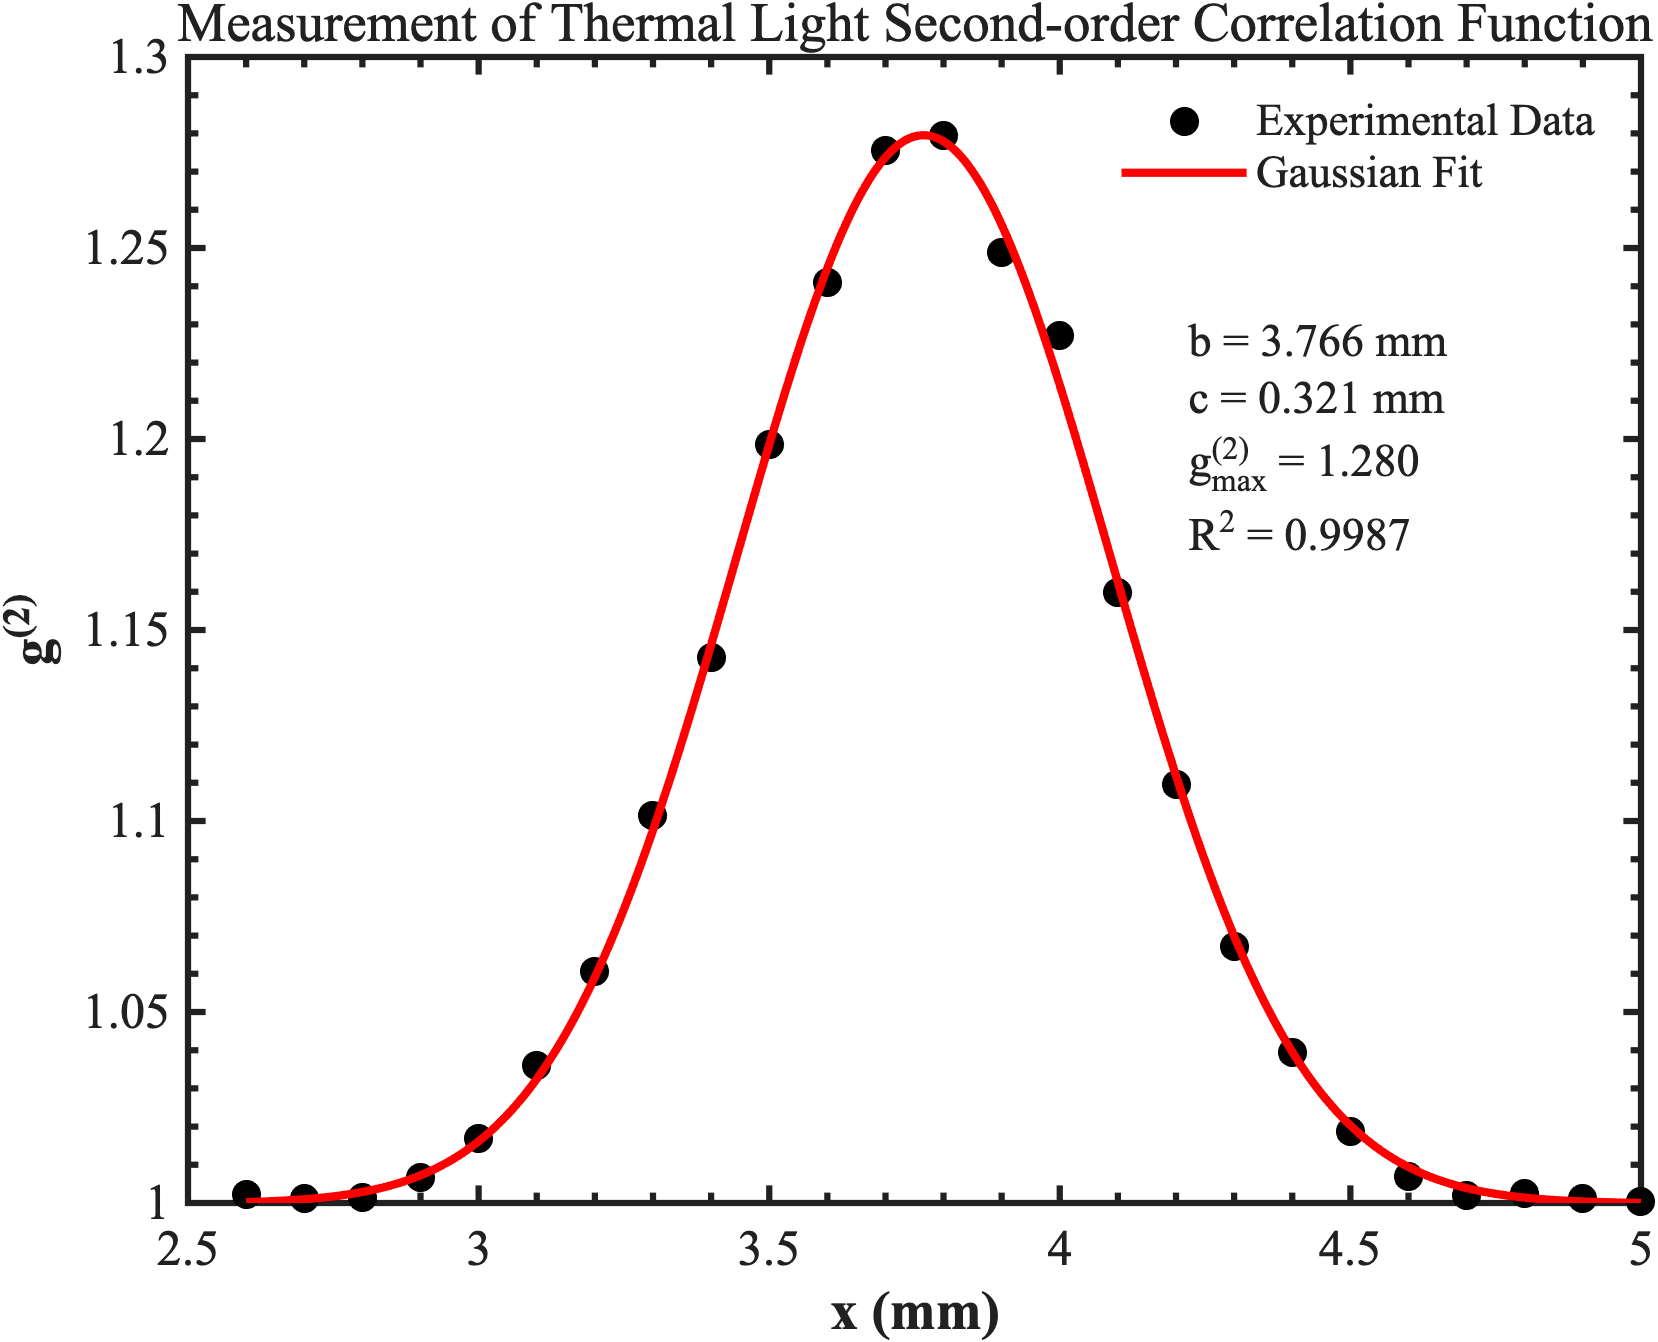
\includegraphics[width=0.75\textwidth]{fig/coherence_length}
    \caption{热光场二阶关联函数测量结果}
    \label{fig:coherence_length}
\end{figure}

实验测得的关联函数在远离中心区域时逐渐趋近于 1，而在中心附近出现明显峰值。测量结果表明，关联函数最大值约为

\begin{equation}
g^{(2)}_{\max}\approx 1.279 ,
\end{equation}

对应的位置约为

\begin{equation}
x_c \approx 3.8~\mathrm{mm}.
\end{equation}

这说明实验成功观测到了热光场的光子聚束效应（photon bunching），即两个探测器同时探测到光子的概率高于完全无关联情形。

对实验数据采用高斯函数

\begin{equation}
g^{(2)}(x)
=
a\exp\left[
-\frac{(x-b)^2}{2c^2}
\right]
+d
\end{equation}

进行拟合，可以得到关联函数的空间分布及对应的关联长度。

% \begin{figure}[htbp]
%     \centering
%     \includegraphics[width=0.75\textwidth]{fig/coherence_fit}
%     \caption{关联函数高斯拟合结果}
%     \label{fig:coherence_fit}
% \end{figure}

拟合结果表明，关联函数具有典型的高斯分布特征，其半高宽对应的空间尺度即为热光场的关联长度。实验结果与热光统计理论的预期一致，说明旋转毛玻璃产生的赝热光具有明显的空间二阶关联特性。

\vspace{0.5em}

\textbf{误差分析}

实验中关联函数峰值未达到理想热光理论值 $g^{(2)}(0)=2$，其主要原因在于实际光源并非理想热光源，同时探测器响应时间有限、光路准直误差以及有限统计时间都会降低测得的关联峰值。此外，机械位移平台的读数误差以及环境振动也会影响关联函数的测量精度。


\subsection{热光关联成像实验}

在取样臂中放置双孔物体，并利用关联成像系统测量参考臂探测器位置与二阶关联函数之间的关系。固定桶探测器后，沿横向扫描参考臂探测器位置，得到关联成像结果。

\begin{figure}[htbp]
    \centering
    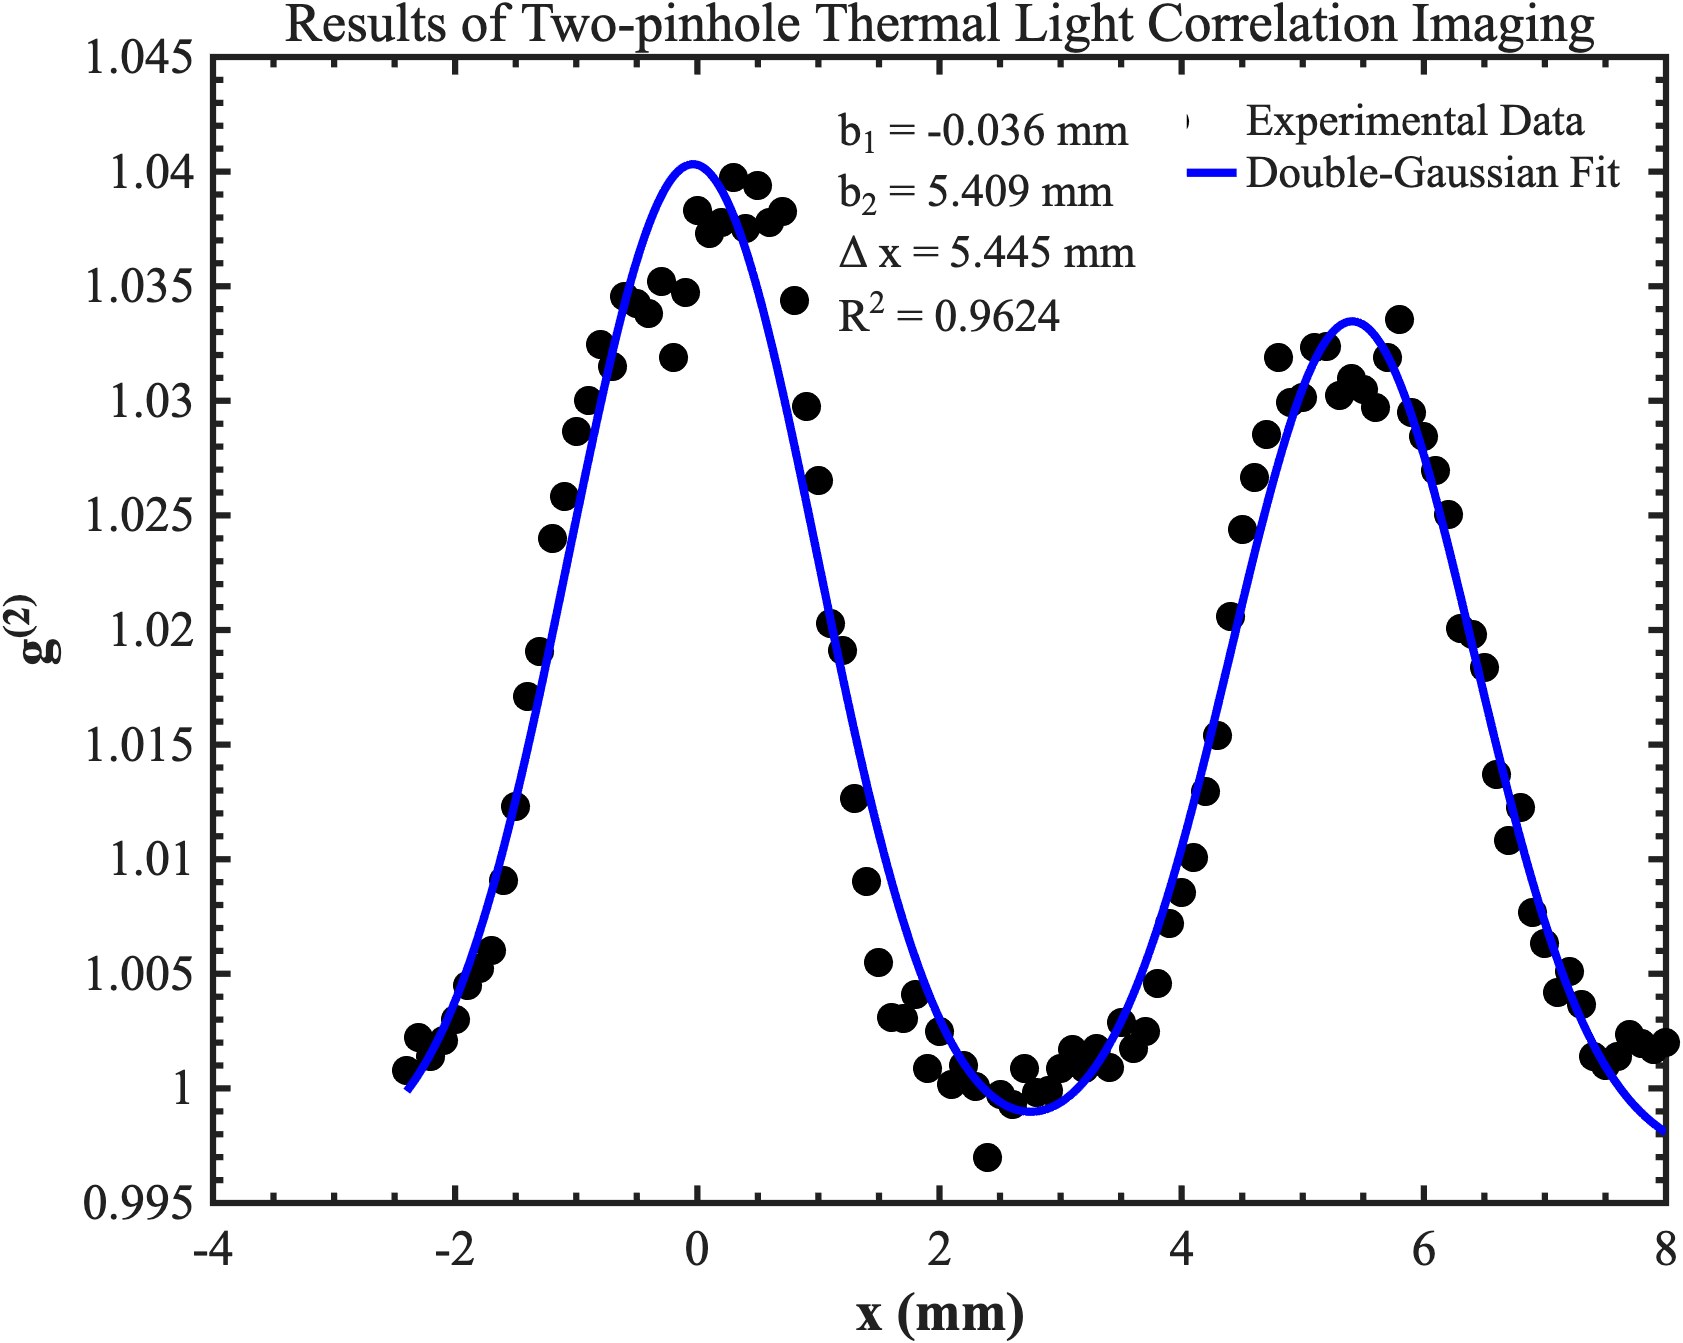
\includegraphics[width=0.75\textwidth]{fig/ghost_image}
    \caption{双孔物体的热光关联成像结果}
    \label{fig:ghost_image}
\end{figure}

实验结果显示，关联函数曲线呈现明显的双峰结构。两个峰分别对应双孔物体的两个透光区域，说明系统成功恢复出了物体的空间信息，实现了热光关联成像。

根据双孔实测尺寸，

\begin{equation}
x_1 = 0.768~\mathrm{cm},
\qquad
x_2 = 0.991~\mathrm{cm},
\end{equation}

可得双孔中心间距为

\begin{equation}
d = x_2-x_1
=0.223~\mathrm{cm}
=2.23~\mathrm{mm}.
\end{equation}

实验获得的关联函数曲线中同样能够清晰观察到两个对应的关联峰，表明关联成像系统能够有效重建双孔物体的信息。虽然成像结果能够定性反映双孔结构，但峰宽相对较大，空间分辨率受到热光关联长度及探测器尺寸的限制，因此得到的关联像相比真实物体存在一定展宽。

\vspace{0.5em}

\textbf{误差分析}

本实验中关联成像结果与理论模型之间存在一定偏差。其中一个重要原因是在实验搭建过程中，将理论成像条件中的

\begin{equation}
z_2-z_1
\end{equation}

误认为

\begin{equation}
z_1-z_2 ,
\end{equation}

导致系统光路未能严格满足热光关联成像的理论条件。因此，实验得到的关联像虽然能够正确反映双孔结构，但其尺度关系与理论放大倍率之间出现了一定偏离。

此外，光路准直误差、透镜安装位置误差以及探测器有限尺寸都会导致关联像发生展宽。由于关联成像本质上依赖于二阶统计量，因此有限采样时间带来的统计涨落也会降低测量精度，使得关联函数曲线出现噪声和波动。

总体而言，实验成功测得了热光场的二阶关联特性，并利用关联函数恢复出了双孔物体的空间结构，验证了热光关联成像的基本原理。
\section{总结}

本实验利用旋转毛玻璃产生类热光源，通过HBT实验测量了热光场的时间关联特性，并进一步实现了双孔物体的热光关联成像。实验结果表明，虽然参考臂和取样臂中的单独光强分布均无法直接反映物体信息，但通过二阶强度关联测量能够恢复物体的空间结构。实验验证了热光场存在空间关联，并验证了热光关联成像所满足的高斯成像公式。

通过本实验，加深了对光场高阶关联性质、HBT实验以及鬼成像原理的理解，也进一步认识到关联测量在现代光学成像中的重要作用。热光关联成像实验表明，部分原本被认为属于量子纠缠体系的成像现象，同样可以利用经典统计关联加以解释和实现。


\end{document}
